\documentclass[10pt]{article}
\usepackage[top=1cm, bottom=1cm, left=1cm, right=1cm]{geometry}
\usepackage{graphicx}
\usepackage{hyperref}
\usepackage{verbatim} 

\title{Eclipse UMC Plugin Readme}
\author{Timotei Dolean}

\begin{document}

\maketitle

\newcounter{cnt}
\newcommand{\icnt}{ \stepcounter{cnt} \thecnt }

\section{Foreword} \hskip\parindent
Through this readme the following terms with the specified meaning will be used:
\begin{enumerate}
\item Project - a directory on the harddrive that is represented as a top directory in the navigator.
\item Container - this is a directory or a project. Basically it can contain any file or directory children.
\item Navigator - an Eclipse view that shows the projects in the workspace
\item Userdata directory - the default directory where wesnoth stores information (addons, preferences, etc)
\end{enumerate}

The following image will highlight the terms used: 1 - Navigator, 2 - Project, 3 - Containers, 4 - Map files, 5 - Config files that contain WML code, 6 - User Addons project.

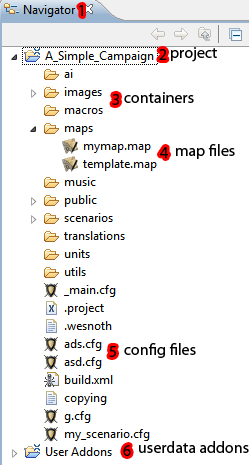
\includegraphics{definitions.png}

\section{Common prerequisites}
\begin{enumerate}
\item Download and install Sun's Java:
\begin{enumerate}
\item If you are going just use it (User): \href{https://cds.sun.com/is-bin/INTERSHOP.enfinity/WFS/CDS-CDS_Developer-Site/en_US/-/USD/ViewProductDetail-Start?ProductRef=jre-6u21-oth-JPR@CDS-CDS_Developer}{Download JRE}
\item If you are going to modify it (Developer): \href{http://java.sun.com/javase/downloads/widget/jdk6.jsp}{Download JDK}
\end{enumerate}
\item Download the  `Eclipse for RCP and RAP Developers" (\href{http://eclipse.org/downloads/packages/eclipse-rcp-and-rap-developers/heliosr}{Download Eclipse}) -
The download links are in the right. Please ensure you are downloading the \textbf{3.6} version,
otherwise the plugin will not work.
\item Extract the downloaded archive in a known location and launch the executable (eclipse / eclipse.exe)
\end{enumerate}

\section{User}
\subsection{Installing the plugin}
\begin{enumerate}
\item After launching Eclipse, go to the ``Help'' menu - Install new Software. \\
  Then, please check ``Group items by category" and ``Contact all update sites during install to find required software", in the bottom of the page.
\item Insert the link \textbf{http://eclipse.wesnoth.org/} in the textbox in the top and press Enter. The list will be populated with some items.
\item Select \textbf{``Wesnoth UMC Plugin"} from the ``eclipse\_plugin" category and press finish.

\textit{Note:} If you are prompted for any license agreements or certificates press Yes on all (if you agree).\\
\textit{Note:} After the plugin has installed, press ``Restart workbench now" when you are prompted.
\end{enumerate}

\section{Developer}
\subsection{Setup the environment}
\begin{enumerate}
\item Checkout plugin's folder from the svn (http://svn.gna.org/svn/wesnoth/trunk/utils/java/) and select the following folders: ``eclipse\_plugin", ``org.wesnoth.wml'', ``org.wesnoth.wml.ui"
\item In Eclipse, right click in \textbf{Package Explorer/Project Navigator} and then select
 \textbf{Import - General - Existing projects into Workspace}
\item Select the path where you downloaded the java folder, and check all the 3 projects: ``eclipse\_plugin", ``org.wesnoth.wml'', ``org.wesnoth.wml.ui".
\item Build the projects.
\end{enumerate}

\subsection{Running the plugin} \hskip\parindent
After you've setup the environment and built the plugin you can run it.
\begin{enumerate}
\item Open the file plugin.xml
\item In the \textbf{Testing} section, select the desired method of launching the plugin
  (non-debug/debug mode).
\end{enumerate}

\section{Everybody}
\subsection{Using the plugin} \hskip\parindent
After you have your plugin installed(user) or running(developer), you can use its features.

But before of all, you must ``Setup the workspace". For this, go in the ``Wesnoth" menu and select ``Setup the workspace". The preferences page for the plugin will pop up, and you must fill them all, so the plugin will work as intended. After you completed the fields, press \textbf{Apply} and then \textbf{OK}. Then the plugin will create a project named ``User addons" in your workspace, which will represent the \textbf{userdata/data/add-ons} directory. 

If there were no errors a message window will open saying: \textbf{Workspace was setup successfully}.\\

\textit{Note:} If you encounter any errors, the plugin logs them in the: \textbf{\textless your temporary directory\textgreater /wesnoth\_plugin}. 
That is usually on linux:\\
\indent \textbf{/tmp/wesnoth\_plugin}\\
or on windows:\\ 
\indent \textbf{C:/Documents and settings/\textless your username\textgreater/Local Settings/Temp/wesnoth\_plugin} \\ 
or\\ 
\indent \textbf{C:/Users/\textless your username\textgreater/Local Settings/Temp/wesnoth\_plugin}

\subsubsection{Wizards} \hskip\parindent
There are some wizards available in the plugin, that will create either projects or config files, based on the specified input. This wizards are available by going to the ``File" menu - New - Other... , and from that list selecting the ``Wesnoth" category.

There are 3 wizards categories:
\begin{enumerate}
\item Project wizards - ``Empty project" and ``Campaign" wizards create new projects in the workspace. The former will create a basic addon directory structure. The latter will create a campaign and it's directory structure.
\item File wizards - ``Scenario", ``Era" and ``Faction" wizards create a new file in a selected container.
\item Wizard launcher - This is a special wizard. It takes a wml tag as input, and generate subsequent needed tags and key inputs. This is generated on the wml schema, so if the schema is incomplete some tags won't be available. This wizard can create a new file or copy the resulted WML into the current edited file.
\end{enumerate}

\subsubsection{Menus} \hskip\parindent
There are currently 2 types of menus: the context menus for different file/container types and the main menu. For a better distinction the menus have the wenoth icon near each item.

\begin{description}
\item{\textbf{Project context menus}} - right click on the projects created with the plugin

   \textit{Wesnoth project report} - will show a simple report with the numer of maps, scenarios and units.\\
   \textit{Upload addon} - will upload the specified directory on the wesnoth addon server. The status will be outputed to the console.

\item{\textbf{Container context menus}} - right click on any container

   \textit{Open campaign in game} - will start the current project's campaign (if any) in wesnoth. For this to work, you must have a ``\_main.cfg" file defined, and a campaign in it.\\
    \textit{WML Tools} - provides some options for using the wmltools with the specified project.

\item{\textbf{``maps" folder context menu}} - right click on the ``maps" directory

   \textit{Import map} - Shows a file selection window that will ley you select a .map file that will be copied in your maps directory.

\item{\textbf{.cfg files context menu}} - right click on any .cfg file

   \textit{Open scenario in game} - opens the selected file's scenario (if it contains one) in wesnoth.\\
   \textit{WML Tools} - provides some options for using the wmltools with the specified file. (e.g. run wmllint against the file and see the output in the console) \\
   \textit{Preprocessor} - provides ways of preprocessing and showing the result in an editor inside eclipse.

\item{\textbf{.map files context menu}} - right click on any .map file\\

   \textit{Open map in editor} - will open the selected map in the wesnoth map editor.

\item{\textbf{Main menu}} - This is a menu near the ``Window" menu bar

   \textit{Open editor} - Will open the game editor with a blank map.\\
   \textit{Open game} - Will open the game.\\
   \textit{Import map} - It will import a map in selected container.\\
   \textit{Open editor} - Open the selected map in the game editor.\\
   \textit{Setup workspace} - Will setup the workspace if it's not setup. This will open the preferences page if any preferences is missing, and then it will create the ``User Addons" project.\\
   \textit{Reload cache} - Reloads the internal cached files. Usefull when the schema or other files have modified and you don't want to restart the plugin.\\
   \textit{Open plugin's preferences} - Opens the plugin preferences page.\\
\end{description}
\end{document}
